\documentclass{beamer}
%[aspectratio=169]   \usepackage[czech]{babel}
\usepackage{apo-lecture}
\usepackage{pdfpages}
\usepackage{pdfcomment}
\usepackage{listings}
\usepackage{array,multirow}

\subtitle{Lekce 01. Úvod}
\author{Pavel Píša \phantom{xxxxxxxxx} Petr Štěpán \\ \small\texttt{pisa@fel.cvut.cz}\phantom{xxxx}\small\texttt{stepan@fel.cvut.cz}}

\begin{document}

\maketitle

\section{Úvod}


\begin{frame}
\frametitle{Motivace}
Co můžete udělat pro zrychlení Vašeho programu:
\begin{itemize}
\item Použít výkonnější počítač:
  \begin{itemize}
  \item Zvýšit výkon CPU 
    \begin{itemize}
    \item Frekvence CPU
    \item Efektivita CPU - kolik operací stihne provést za 1 takt procesoru
    \end{itemize}
  \end{itemize}
\item Změnit program:
  \begin{itemize}
  \item Zlepšit efektivitu práce s pamětí
  \item Paralelizovat program:
    \begin{itemize}
    \item Zvýšit počet jader CPU
    \end{itemize}
  \end{itemize}
\end{itemize}
\end{frame}


\begin{frame}
\frametitle{Motivace}
Má paralelizace nějaká omezení:
\begin{itemize}
\item Nikdy nelze paralelizovat celý program
\item Amdahlův zákon
  \begin{itemize}
  \item $\alpha$ procent programu nelze paralelizovat
  \item zbytek programu $1-\alpha$ lze na $p$ procesorech zrychlit na $\frac{1 - \alpha}{p}$
  \item Poměr zrychlení na $p$ procesorech $S(p) = \frac{\alpha + 1 - \alpha}{\alpha + \frac{1-\alpha}{p}} = \frac{p}{1+\alpha \cdot (p-1)}$
  \item Limit zrychlení je pro nekonečně procesorů $S(p\to\infty) = lim_{p\to\infty}\frac{p}{1+\alpha \cdot (p-1)} = \frac{1}{\alpha}$
    \begin{itemize}
    \item Např pro $\alpha=0.3$ je limit $S(p\to\infty) = 3.\overline{3}$, tedy program nelze zrychlit více než $3.\overline{3}$ krát. 
    \end{itemize}
  \end{itemize}
\item V praxi, čím více máte procesů, tím stoupá i náročnost přípravy dat pro paralelizaci.
\end{itemize}
\end{frame}


\begin{frame}
\frametitle{Motivace}
Proč studovat architektury počítačů:
\begin{itemize}
\item Naučit se jak pracuje počítač, který vykonává Váš program a kde jsou možnosti program zefektivnit 
  \begin{itemize}
  \item zjistit, v čem současný počítač zpomaluje výpočet (rychlost procesoru, velikost vyrovnávací paměti, latence hlavní paměti, počet výpočetních jader) a otestovat jiný HW
  \item zjistit, zda lze program upravit, aby využíval lépe dostupné prostředky 
  \begin{itemize}
    \item upravit pořadí přístupu do paměti a tím lépe využívat vyrovnávací paměť
    \item upravit program, aby požíval méně skoků a tím se vykonával rychleji
    \item paralelizovat výpočet, využít specializovaný HW - GPU, externí výpočetní jednotku např. Coral USB nebo Intel Neural Compute Stick~2.
  \end{itemize}
\end{itemize}
\item Poptávka po absolventech kombinující umělou inteligenci a vestavné systémy (embedded system)
\item Pokud je pro Vás počítač BlackBox, pak jsou Vaše programy neefektivní
\end{itemize}
\end{frame}


\begin{frame}
\frametitle{Obsah přednášek}
Projdeme si všechny základní součásti počítače:
\begin{itemize}
\item CPU
\item Hierarchie paměti - Cache/RAM/Disk
\item Vstupy a výstupy - I/O klávesnice, myš, obrazovka, síťová karta, ovladače HW
\item Výjimky a přerušení - efektivní spolupráce CPU s HW
\end{itemize}

Motivace proč navštěvovat přednášky:
\begin{itemize}
\item Něco se naučíte a budete to mít lehčí při přípravě na zkoušku
\item Kdo správně zodpoví kvízovou otázku v závěru přednášky, dostane bod aktivity
  \begin{itemize}
  \item Né každá přednáška, první bodovaný kvíz příští týden 
  \item Celkem 8 bodů za aktivitu na přednáškách
  \end{itemize}
\end{itemize}

\end{frame}

\begin{frame}
\frametitle{Náplň cvičení}

\begin{columns}
\begin{column}{0.6\textwidth}
\begin{itemize}
\item 4 menší domácí úkoly - 36 bodů
\begin{itemize}
\item 2 programy v C
\item 2 formuláře
\item alespoň 3 úlohy ze 4
\end{itemize}
\item Semestrální úloha - 24 bodů
\begin{itemize}
\item Týmový projekt - dvojice, nebo jednotlivci
\item Speciální HW MZ APO deska
\end{itemize}
\end{itemize}
\end{column}
\begin{column}{0.35\textwidth}  
   \begin{tabular}{|l|l|}\hline
   Známka & Body\\ \hline
   A & >=90\\ \hline
   B & 80 -- 89.9\\ \hline
   C & 70 -- 79.9\\ \hline
   D & 60 -- 69.9\\ \hline
   E & 50 -- 59.9\\ \hline
   F & <50\\ \hline
   \end{tabular}
\end{column}
\end{columns}
\begin{itemize}
\item Nepovinné úlohy nebo aktivita při cvičení/přednáškách - 10 bodů
\end{itemize}
\bigskip
Zkouška: 
\begin{itemize}
\item písemný test 30 bodů, min 15 bodů
\item ústní $\pm$ 10 bodů    
\end{itemize}

\end{frame}


\begin{frame}
\frametitle{Navazující předměty}
Pokud Vás tento předmět zaujme, tak na něj navazují tyto předměty:
\begin{itemize}
\item B4M35PAP - Pokročilé architektury počítačů
\item B3B38VSY - Vestavné systémy
\item B4M38AVS - Aplikace vestavných systémů
\item B4B35OSY - Operační systémy
\item B0B35LSP - Logické systémy a procesory
\end{itemize}
\end{frame}


\begin{frame}
\frametitle{Materiály k předmětu}
\begin{itemize}
\item PATTERSON, David A. a John L. HENNESSY. Computer organization and design RISC-V edition:
    the hardware/software interface. Second Edition. Cambridge: Elsevier, [2021].
    ISBN 978-0-12-820331-6. (12 kusů v ústřední knihovně ČVUT)
\item web:
\begin{itemize}
\item https://cw.fel.cvut.cz/b192/courses/b35apo/
\item https://dcenet.felk.cvut.cz/apo/
\end{itemize}
\item Kurzy v angličtině:
\begin{itemize}
\item MIT 6.004/6.191 – Computation Structures
\item Computation Structures | Electrical Engineering and Computer Science | MIT OpenCourseWare (2015)
\item Computer System Architecture | Electrical Engineering and Computer Science | MIT OpenCourseWare (2005)
\end{itemize}
\item Kurzy v češtině:
\begin{itemize}
\item https://courses.fit.cvut.cz/BI-APS/
\item https://www.vut.cz/studenti/predmety/detail/218515?apid=218515
\end{itemize}

\end{itemize}
\end{frame}

\section{Složení počítače}
\begin{frame}
\frametitle{Co je uvnitř počítače}

Základní deska počítače:
\begin{center}
   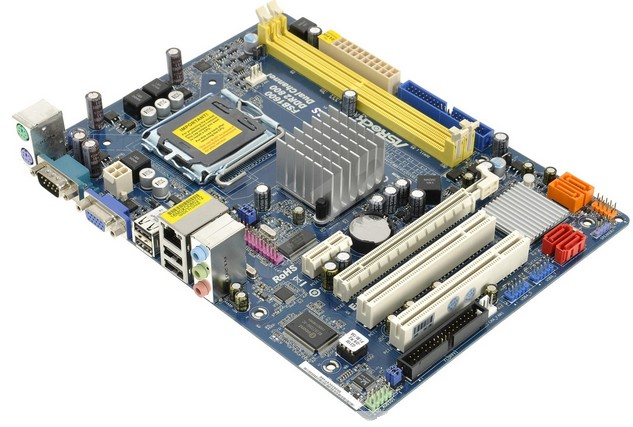
\includegraphics[width=0.8\textwidth]{fig/motherboard.jpg}
\end{center}

\end{frame}

\begin{frame}
\frametitle{Co je uvnitř počítače}

Rozebraný telefon:
\begin{center}
   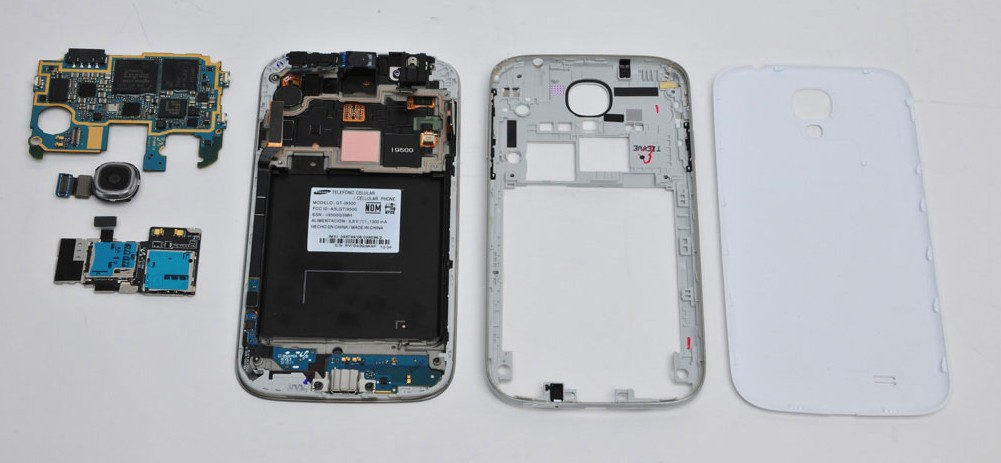
\includegraphics[width=0.6\textwidth]{fig/mobile.jpg}
\end{center}
\begin{center}
   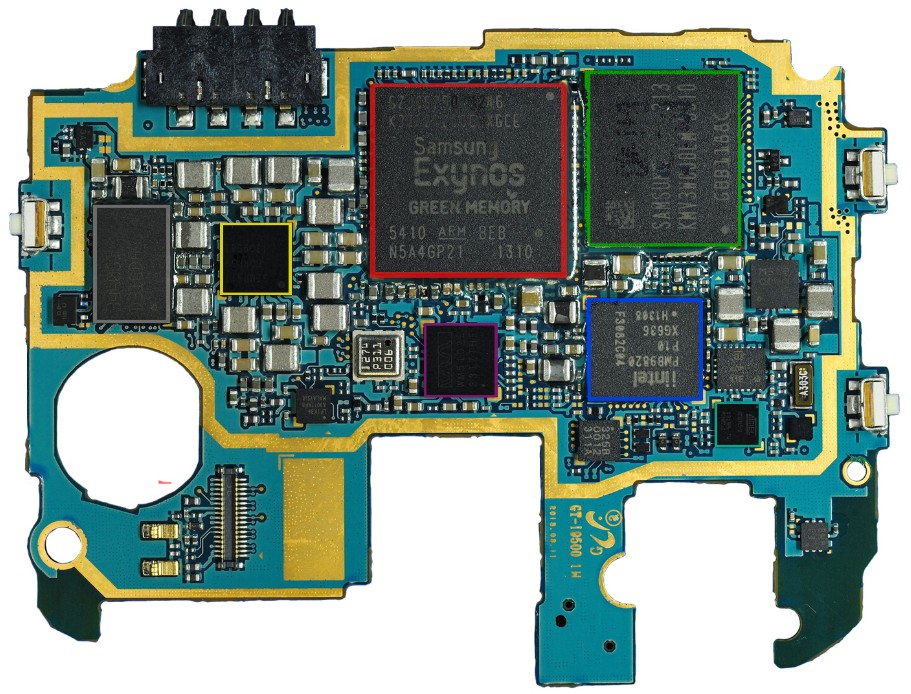
\includegraphics[width=0.4\textwidth]{fig/mobile-cpu.jpg}
\end{center}
\end{frame}


\begin{frame}
\frametitle{von Neumann}

Společný koncept navržený maďarským fyzikem Johnem von Neumannem (1903-1957) obsahuje:
\begin{itemize}
\item Procesor - Central Processing Unit - CPU
\item Paměť - Memory, Random-access Memory, 
\item Vstup/Výstup - Input/Output
\end{itemize}
\begin{center}
   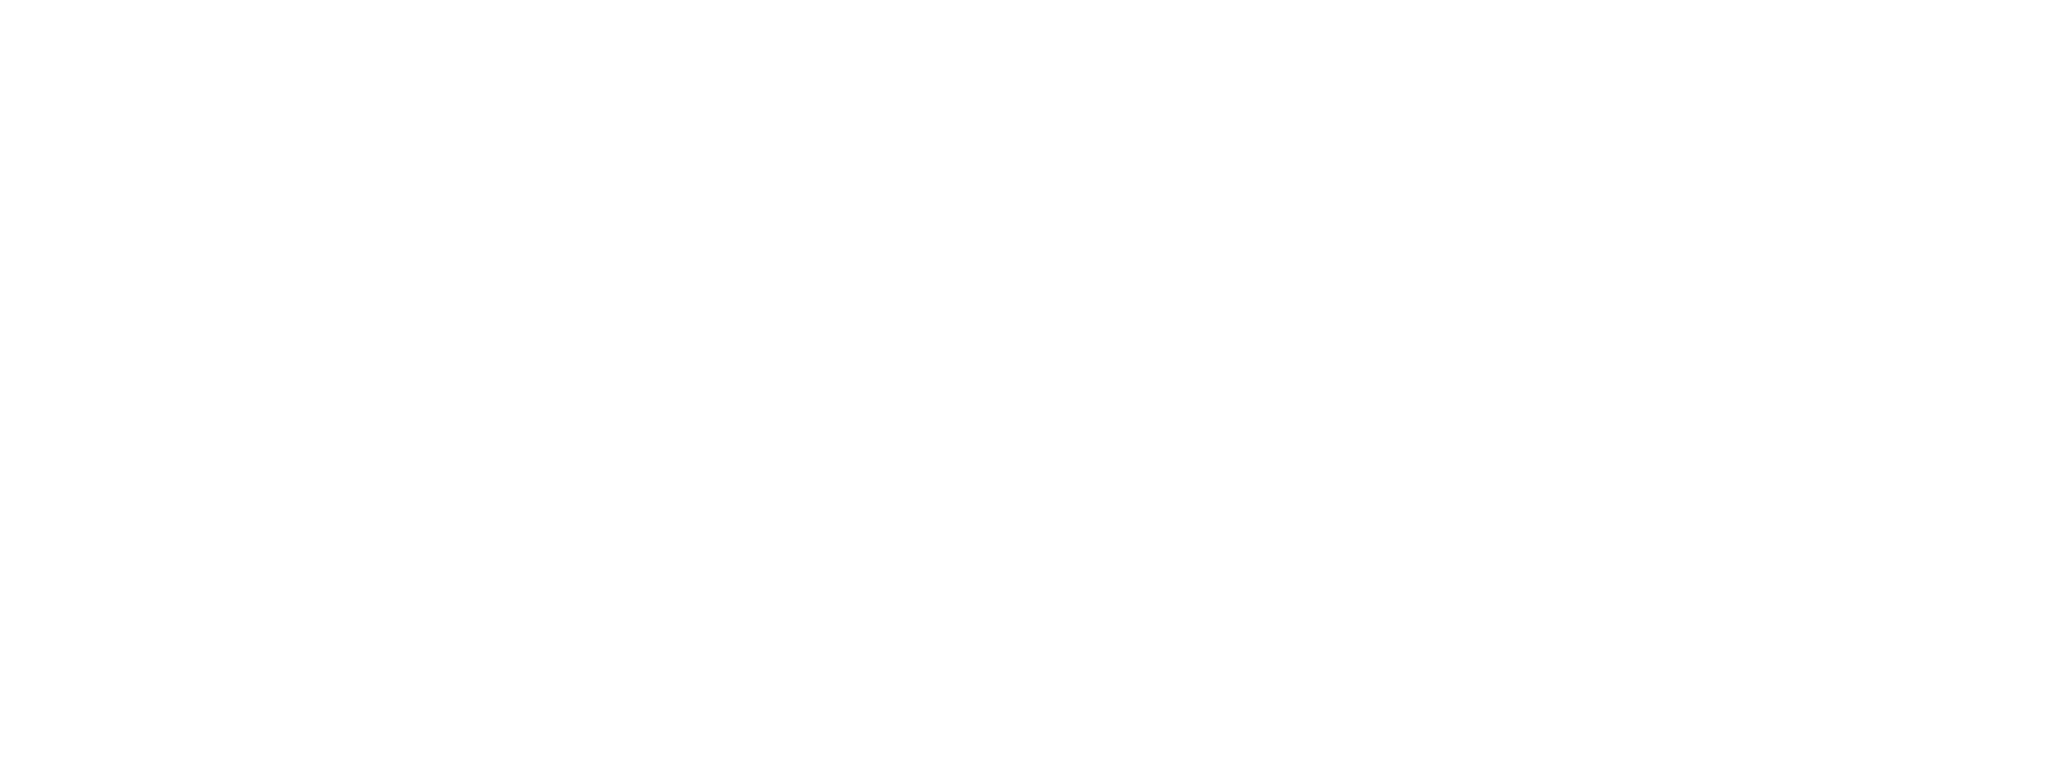
\includegraphics[width=0.7\textwidth]{cpu-vonNeumann.pdf}
\end{center}

\end{frame}


\begin{frame}
\frametitle{CPU}
\begin{columns}
\begin{column}{0.5\textwidth}
\begin{itemize}
\item CPU obsahuje uživatelské registry, které obsahují 16, 32 nebo 64 bitové hodnoty podle architektury čipu
\item CPU načítá z paměti instrukce tak jak jdou za sebou a každou načtenou instrukci vykoná
\item Adresa právě vykonávané instrukce je ve speciálním registru PC nebo IP
\item ALU část CPU která umí sčítat, odčítat, násobit, dělit a další aritmetické operace
\end{itemize}
\end{column}
\begin{column}{0.5\textwidth}  
\begin{center}
   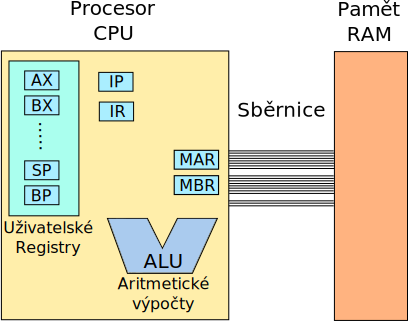
\includegraphics[width=0.95\textwidth]{cpu.pdf}
\end{center}
\end{column}
\end{columns}

\end{frame}



\begin{frame}
\frametitle{Paměť}

Paměť si pamatuje data - bajty, slova.

Pokud už znáte nějaký programovací jazyk, tak si ji můžete představit jako pole, např. v jazyce C jako:\\
\texttt{unsigned char RAM[16 * 1024 * 1024 *1024]; // 16GiB RAM}

\bigskip
Z paměti lze číst:\\
\texttt{registr R10 = RAM[adresa];}\\
nebo zapisovat:\\
\texttt{RAM[adresa] = R10;}

\end{frame}

\begin{frame}
\frametitle{Instrukce procesoru}

\begin{itemize}
\item Instrukce procesoru jsou jediné činnosti, které procesor umí vykonat
\item Základní instrukce jsou:
\begin{itemize}
\item uložit konstantu do registru
\item načíst data z paměti do registru
\item provést matematickou operaci s registry a výsledek uložit do registru
\item uložit data z registru do paměti
\item porovnat dvě čísla
\item podle výsledku porovnání provádět jiné instrukce (změnit PC na jinou hodnotu než je následující instrukce = provést skok v programu)
\end{itemize}
\item veškeré programy, ať už vytvořené v jazyku C, Python, programy provádějící i velmi komplexní výpočty jsou složené pouze z těchto jednoduchých instrukcí procesoru
\end{itemize}

\end{frame}

\begin{frame}
\frametitle{Instrukce procesoru}

Instruction Set Architecture (ISA) Architektura souboru instrukcí
\begin{itemize}
\item je kompletní instrukční sada včetně adresních módů
\item např. x86 (IA-32), x86-64 (AMD64, EM64T, IA-32e), ARM32, ARM64, AVR, MIPS, RISC-V
\item ISA obsahuje:
\begin{itemize}
\item množinu strojových instrukcí procesoru
\item podporované datové typy (celá čísla, celá čísla se znaménkem, reálná čísla)
\item množina registrů
\item adresní módy
\item organizace paměti
\end{itemize}
\end{itemize}

\end{frame}


\begin{frame}
\frametitle{Instrukce procesoru}

Dva základní přístupy k návrhu ISA
\begin{columns}
\begin{column}{0.5\textwidth}
\begin{center}
\LARGE{RISC}
\end{center}
Reduced Instruction Set Computer
\begin{itemize}
\item Obvykle menší počet instrukcí
\item Všechny instrukce mají stejný počet bajtů, některé umožňují poloviční délku
\item Méně jednodušších adresních módů
\item Matematické operace ALU pouze s registry
\end{itemize}
\end{column}
\begin{column}{0.5\textwidth}  
\begin{center}
\LARGE{CISC}
\end{center}
Complex Instruction Set Computer
\begin{itemize}
\item Obvykle větší počet instrukcí
\item Délka instrukcí je od 1 bajtu do např. 12 bajtů, nejčastější instrukce jsou nejkratší
\item Obvykle mnoho i složitých adresních módu
\item Matematické oprace ALU i s hodnotami z paměti
\end{itemize}

\end{column}
\end{columns}
\end{frame}


\begin{frame}
\frametitle{Překlad programu}

Jak je možné, že jste o strojových instrukcích ještě neslyšeli?

\begin{center}
   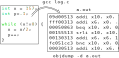
\includegraphics[width=0.65\textwidth]{preklad.pdf}
\end{center}

\begin{itemize}
\item Programování v assembleru (jazyku symbolických adres) je nekomfortní.
\item Překladač přeloží vyšší programovací jazyk přímo do strojových instrukcí procesoru
\item Křízový překlad je, když přeložíte program pro jiný typ procesoru, než na kterém probíhá překlad.
\end{itemize}
\end{frame}



\begin{frame}
\frametitle{Procesor}

Z čeho se vlastně procesor skládá?
\begin{itemize}
\item Možná jste někdy slyšeli, že procesor obsahuje třeba 16 miliard tranzistorů
\item V roce 1965 spoluzakladatel společnosti Intel Gordon Moor formuloval zákon: 
\begin{itemize}
\item Počet tranzistorů, které mohou být umístěny na integrovaný obvod se při zachování stejné ceny zhruba každých 18 měsíců zdvojnásobí.
\end{itemize}
\item Více méně platí až do dnes, i když už se dostáváme na hranice fyzikálních možností.
\end{itemize}

K čemu potřebujeme v procesoru = CPU tranzistory?
\begin{itemize}
\item Abychom implementovali Booleovu algebru.
\end{itemize}
\end{frame}



\section{Boolova algebra}



\begin{frame}
\frametitle{Booleova algebra}

Booleova algebra je matematická struktura:
\begin{itemize}
\item Používá pouze dvě hodnoty 0,1
\begin{itemize}
\item 0/1, nebo False/True, nebo nesvítí/svítí, nebo 0V/5V
\end{itemize}
\item Operace plus (nebo, ||, or, $\lor$)
\begin{itemize}
\item 0+0=0 \phantom{XXXX}  0+1=1
\item 1+0=1 \phantom{XXXX}  1+1=1
\end{itemize}
\item Operace krát (a, \&\&, and, $\land$)
\begin{itemize}
\item 0*0=0 \phantom{XXXX}  0*1=0
\item 1*0=0 \phantom{XXXX}  1*1=1
\end{itemize}
\item Operace inverzní prvek - (negace, !, not, $\neg$)
\begin{itemize}
\item -0 = 1
\item -1 = 0
\end{itemize}
\end{itemize}
\end{frame}


\begin{frame}
\frametitle{Boolova algebra}

Booleova algebra se dá dobře implementovat pomocí napětí a tranzistorů (nebude u zkoušky)

\begin{columns}
\begin{column}{0.45\textwidth}
Napětí jednoho vodiče vůči zemi definuje logickou hodnotu.
\end{column}
\begin{column}{0.55\textwidth}  
\begin{center}
   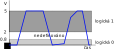
\includegraphics[width=0.9\textwidth]{ttl_log01.pdf}
\end{center}
\end{column}
\end{columns}

\begin{columns}
\begin{column}{0.45\textwidth}
Příklad: Logická operace not, jeden vstupní vodiče X, jeden výstupní vodič Y.
\end{column}
\begin{column}{0.55\textwidth}  
\begin{center}
   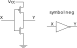
\includegraphics[width=0.8\textwidth]{cmos_neg.pdf}
\end{center}
\end{column}
\end{columns}


%inkscape ctrl shift Y logic symbols
\end{frame}

\begin{frame}
\frametitle{Booleova algebra}

Rozšířené operace \texttt{nand}, \texttt{nor}, \texttt{xor} a libovolné logické funkce se skládají ze základních operací (\texttt{and}, \texttt{or}, \texttt{not}):

\begin{tabular}{ll}
\texttt{X nand Y} & \texttt{= not(X and Y)}\\
\texttt{X nor Y} & \texttt{= not(X or Y)}\\
\texttt{X xor Y} & \texttt{= (X or Y) and (not(X and Y))}\\
& \texttt{= (X or Y) and (X nand Y)}\\
\end{tabular}


\end{frame}


\begin{frame}
\frametitle{Booleova algebra}

Přehled hradel a jejich symbolů
\begin{center}
   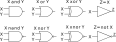
\includegraphics[width=0.8\textwidth]{log_symbols.pdf}
\end{center}

Souhrná tabulka základních logických hradel:
\begin{tabular}{|c|c|c|c|c|c|c|c|}\hline
X & Y & X and Y & X or Y & X xor Y & X nand Y & X nor Y & X xnor Y \\\hline
0 & 0 &    0    &   0    &    0    &     1    &    1    &    1     \\\hline
0 & 1 &    0    &   1    &    1    &     1    &    0    &    0     \\\hline
1 & 0 &    0    &   1    &    1    &     1    &    0    &    0     \\\hline
1 & 1 &    1    &   1    &    0    &     0    &    0    &    1     \\\hline
\end{tabular}

\end{frame}


\begin{frame}
\frametitle{Booleova algebra - kvíz}

Vodiče se mohou i větvit. Co dělá následující obvod:
\begin{center}
   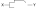
\includegraphics[width=0.4\textwidth]{not_jako_nand.pdf}
\end{center}

\begin{tabular}{ll}
A) takto to nelze zapojit \phantom{XXXX} & B) výsledkem je X and Y\\
C) výsledkem je X and not Y              & D) výsledkem je not X
\end{tabular}

\end{frame}


\begin{frame}
\frametitle{Logické obvody}

Některé funkce lze převést do hradel i efektivněji než přes základní logické funkce and, or, not.

Hradlo nand je základním hradlem a lze z něj postavit všechny ostatní hradla.

\begin{center}
   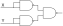
\includegraphics[width=0.5\textwidth]{or_by_nand.pdf}
\end{center}

Kvíz: Co je toto za funkci:
\begin{itemize}
\item[A] X and Y
\item[B] X or Y
\item[C] X xor Y
\item[D] X nor Y
\end{itemize}

\end{frame}


\begin{frame}
\frametitle{Logické obvody}

\begin{columns}
\begin{column}{0.55\textwidth}
Logické obvody jsou složitější obvody složené ze základních logických členů - hradel. Signály se mohou větvit, spojují se vždy nějakou logickou operací.
Výsledkem logického obvodu jsou vždy jen logické hodnoty 0 nebo 1.

\bigskip

Kvíz: Co dělá tento obvod:
\begin{itemize}
\item[A] Nic rozumného, je to jen spleť vodičů
\item[B] Je to multiplexor, hodnota Z je jeden ze signálů X podle hodnoty Y
\item[C] Je to dělička, hodnota Z je X/Y
\item[D] Hodnota Z je 1 pokud je X > Y 
\end{itemize}
\end{column}
\begin{column}{0.45\textwidth}  
\begin{center}
   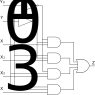
\includegraphics[width=0.95\textwidth]{multiplex.pdf}
\end{center}
\end{column}
\end{columns}


\end{frame}


\begin{frame}
\frametitle{Binární soustava - kvíz}

Kvíz: Jeden vodič reprezentuje jednu hodnotu, buď 0 nebo 1. Jak reprezentovat více hodnot, třeba všechna celá čísla od 0 do 255 (tedy jeden bajt):
\begin{itemize}
\item[A] Jeden vodič má 8 rozdílných úrovní napětí
\item[B] Jeden vodič reprezentuje postupně v čase 8 různých hodnot 0/1
\item[C] Osm vodičů, každý reprezentuje v jeden čas jednu z hodnot 0/1
\item[D] 256 vodičů, pouze jeden má hodnotu 1 ostatní 
\end{itemize}


\end{frame}


\begin{frame}
\frametitle{Binární soustava}

Více bitová čísla - binární soustava
\begin{itemize}
\item více jednobitových paralelních vodičů
\begin{itemize}
\item zpravidla 8,16,32,64 (mocniny 2)
\item občas potřebujeme i jen části čísel, třeba 5-bitové
\end{itemize}
\item pořadí vodičů je důležité
\begin{itemize}
\item každý vodič reprezentuje jednu mocninu 2
\item vodič $a_{i}$, celková hodnota $s = \sum_{i=0}^{63} a_{i}*2^{i}$
\end{itemize}
\end{itemize}

\end{frame}


\begin{frame}
\frametitle{Sčítání}

Součet dvou jednobitových čísel:
\begin{tabular}{|r|r|c|}\hline
X & Y & X+Y\\ \hline
0 & 0 & 00\\ \hline
0 & 1 & 01\\ \hline
1 & 0 & 01\\ \hline
1 & 1 & 10\\ \hline
\end{tabular}

\bigskip

\begin{columns}
\begin{column}{0.55\textwidth}
Výsledek součtu může být dvoubitové číslo $C$ - přenos, $S$ - součet.
\bigskip

\texttt{$S$ = $X$ xor $Y$}\\
\texttt{$C$ = $X$ and $Y$}

\bigskip

Tomuto logickému obvodu se říká poloviční sčítačka (Half adder)
\end{column}
\begin{column}{0.45\textwidth}  
\begin{center}
   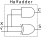
\includegraphics[width=0.75\textwidth]{half_adder.pdf}
\end{center}
\end{column}
\end{columns}

\end{frame}

\begin{frame}
\frametitle{Sčítání}

Pokud sčítáme vícebitová čísla potřebujeme později sečíst tři bitové vstupy.

\begin{columns}
\begin{column}{0.6\textwidth}
Výsledek součtu je opět dvoubitové číslo: $C_{out}$~-~přenos, $S$~-~součet.

\begin{columns}
\begin{column}{0.55\textwidth}

\bigskip

\begin{tabular}{|r|r|r|c|}\hline
C & X & Y & C+X+Y\\ \hline
0 & 0 & 0 & 00\\ \hline
0 & 0 & 1 & 01\\ \hline
0 & 1 & 0 & 01\\ \hline
0 & 1 & 1 & 10\\ \hline
1 & 0 & 0 & 01\\ \hline
1 & 0 & 1 & 10\\ \hline
1 & 1 & 0 & 10\\ \hline
1 & 1 & 1 & 11\\ \hline
\end{tabular}

\end{column}
\begin{column}{0.45\textwidth}

\texttt{$S_1$ = ($X$ xor $Y$)}\\
\texttt{$S$ = ($S_1$ xor $C$)}\\
\texttt{$C_1$ = ($X$ and $Y$)}\\
\texttt{$C_2$ = ($S_1$ and $C$)}\\
\texttt{$C_{out}$ = $C_1$ or $C_2$}

\bigskip

Tomuto logickému obvodu se říká úplná sčítačka 

(Full adder)
\end{column}
\end{columns}

\end{column}
\begin{column}{0.4\textwidth}  

\begin{center}
   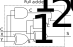
\includegraphics[width=\textwidth]{full_adder.pdf}
\end{center}


\begin{center}
   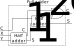
\includegraphics[width=\textwidth]{full_adder2.pdf}
\end{center}

\end{column}
\end{columns}


\end{frame}

\begin{frame}
\frametitle{Sčítání - Ripple Carry Adder}

Nejjednodušší sčítačka vícebitových čísel prostě propojí jednu poloviční sčítačku a plné sčítačky. 

Tato sčítačka se jmenuje Ripple Carry Adder (Řetězová sčítačka).

\begin{center}
   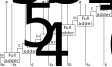
\includegraphics[width=0.7\textwidth]{ripple_adder.pdf}
\end{center}

$a_5a_4a_3a_2a_1a_0 + b_5b_4b_3b_2b_1b_0 = s_6s_5s_4s_3s_2s_1s_0$ platí, že $s_6 = c_6$

\end{frame}

\begin{frame}
\frametitle{Sčítání - Ripple Carry Adder}

Jak rychlá je Ripple Carry Adder?
\begin{itemize}
\item Pokud je zpoždění jednoho hradla N pak zpoždění Ripple Carry Adder pro dvě 64-bitové hodnoty 63*3*N+2*N
\item Je to důležité?
\begin{itemize}
\item Ano, při taktu CPU 4GHz trvá jeden takt 250 ps (pikosekund)
\item Omezení je i rychlost světla 0.3 mm/ps, to je maximální rychlost šíření informace
\item Při zpoždění hradla kolem 10ps, pak Ripple Carray Adder by sečetla 2 čísla za 1910ps  
\end{itemize}
\item Lze to rychleji?
\begin{itemize}
\item Ano, Carry Lookahead adder
\end{itemize}
\end{itemize}

\end{frame}

\begin{frame}
\frametitle{Sčítání - Carry Lookahead adder}

\begin{itemize}
\item Lze spočítat $C_1$, $C_2$, ... , rovnou ze sčítaných čísel?
\begin{itemize}
\item Ano, ale pro hodně bitová čísla to je drahé, potřebujeme hodně hradel.
\item Ukážeme si to pro 4-bitová čísla
\item Nadefinujeme si dvě základní hodnoty:
\begin{itemize}
\item Generování carry -- pokud $A_i=1$ a $B_i=1$ pak určitě bude $C_{i+1}=1$ tedy carry se vygeneruje $G_i=A_i \land B_i$ 
\item Propagování carry -- pokud $A_i=1$ nebo $B_i=1$ pak bude $C_{i+1}=C_{i}$ tedy carry se bude propagovat, pokud bylo nižší carry; $P_i=A_i$ xor $B_i$ 
\end{itemize}
\item Pro 4-bitové číslo:
\begin{itemize}
\item $C_1=G_0$ 
\item $C_2=G_1 \lor (C_1 \land P_1)= G_1 \lor (G_0 \land P_1)$
\item $C_3=G_2 \lor (C_2 \land P_2)= G_2 \lor (G_1 \land P_2) \lor (G_0 \land P_1 \land P_2)$ 
\item $C_4=G_3 \lor (C_3 \land P_3)= G_3 \lor (G_2 \land P_3) \lor (G_1 \land P_2 \land P_3) \lor (G_0 \land P_1 \land P_2 \land P_3)$
\item takto bychom mohli pokračovat, ale výraz by byl složitější a složitější
\end{itemize}
\end{itemize}
\end{itemize}

\end{frame}

\begin{frame}
\frametitle{Sčítání - Carry Lookahead Adder}

Takto bude vypadat nejrychlejší sčítačka pro 4-bitová čísla. 

Dvě čísla sečte na 4 zpoždění hradla.
\begin{center}
   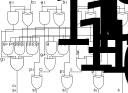
\includegraphics[width=0.65\textwidth]{lookahead_direct.pdf}
\end{center}

Pro 64 bitová čísla by potřebovala sčítačka kolem $10^{20}$ hradel, což je moc.
\end{frame}



\begin{frame}
\frametitle{Sčítání - Carry Lookahead Adder}

Co tedy s většími čísly, třeba 64-bitovými?

\begin{columns}
\begin{column}{0.45\textwidth}
\begin{itemize}
\item Upravíme 4-bitovou sčítačku tak, aby mohla přijmout $C$ z předchozích výpočtů
\begin{itemize}
\item POZOR budou se muset přidat hradla
\end{itemize}
\item Takto upravené sčítačky můžeme řetězit.
\end{itemize}
\end{column}
\begin{column}{0.55\textwidth}
\begin{center}
   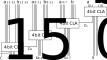
\includegraphics[width=0.95\textwidth]{lookahead_ripple.pdf}
\end{center}
\end{column}
\end{columns}


\begin{itemize}
\item Rychlost 16-ti bitové sčítačky z obrázku bude 16 zpoždění hradel
\item Rychlost 64-ti bitové sčítačky bude 64 zpoždění hradel, což je daleko lepší, než 191 zpoždění u jednoduché Ripple carry adder.
\end{itemize}

\end{frame}


\begin{frame}
\frametitle{Sčítání - Carry Select Adder}


Jiné řešení?

\begin{itemize}
\item Víme, že Carry je buď 0 nebo 1
\item 4bit CLA zdvojíme a spočteme výsledek pokud vstupní Carry je 0 i 1
\item Nakonec řetězíme pouze multiplex, zda skutečně Carry bylo 0 nebo 1
\end{itemize}
\begin{center}
   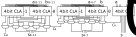
\includegraphics[width=0.75\textwidth]{lookahead_select.pdf}
\end{center}

\begin{itemize}
\item Sčítačka je rychlejší, místo zpoždění 4 hradel bude řetězit pouze zpoždění 2 hradel pro multiplexor
\item Rychlost 16-ti bitové sčítačky z obrázku bude 10 zpoždění hradel
\item Rychlost 64-ti bitové sčítačky bude 34 zpoždění hradel, což je o něco lepší, než 64 zpoždění u řetězení CLA.
\end{itemize}

\end{frame}




\begin{frame}
\frametitle{Sčítání - Carry Lookahead Adder}

Můžeme ještě něco vylepšit?
\begin{itemize}
\item Můžeme zavést proměnné generuj a propaguj pro skupinu bitů:
\begin{itemize}
\item Pokud budou bity $i$ až $j$ generovat přenos (carry), pak $G_{i,j}=1$
\item Pokud budou bity $i$ až $j$ propagovat přenos (carry), pak $P_{i,j}=1$
\end{itemize}
\item Nyní si definujeme pravidla, jak $G_{i,k}$ a $P_{i,k}$ spočítat z $G_{i,j}$, $G_{j+1,k}$,$P_{i,j}$, $P_{j+1,k}$
\begin{itemize}
\item $G_{i,k}=G_{j+1,k} \lor (G_{i,j} \land P_{j+1,k})$
\item $P_{i,k}=P_{i,j} \land P_{j+1,k}$
\end{itemize}
\item Počáteční hodnoty jsou staré známé $G_i$ a $P_i$. 
\item Tedy $G_{i,i}=G_i=a_i \land b_i$ a $P_{i,i}=P_i=a_i$ xor $b_i$.
\end{itemize}

\end{frame}

\begin{frame}
\frametitle{Sčítání - Carry Lookahead Adder}

Takto lze realizovat výše uvedený výpočet:
\begin{columns}
\begin{column}{0.55\textwidth}
\begin{center}
   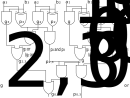
\includegraphics[width=0.95\textwidth]{lookahead_tree.pdf}
\end{center}
\end{column}
\begin{column}{0.45\textwidth}

Doba výpočtu dvojic $G_{i,k}$ a $P_{i,k}$:
\begin{itemize}
\item Rychlost 4 bitových sčítanců 5 zpoždění hradel
\item Rychlost 8 bitových sčítanců 7 zpoždění hradel
\item Rychlost 16 bitových sčítanců 9 zpoždění hradel
\item Rychlost 32 bitových sčítanců 11 zpoždění hradel
\item Rychlost 64 bitových sčítanců 13 zpoždění hradel
\end{itemize}

\end{column}
\end{columns}

\end{frame}


\begin{frame}
\frametitle{Sčítání - Carry Lookahead Adder}

Nyní nám zbývá vypočítat všechny Carry $C_i$, pokud bychom předpokládali řetězení, tak známe $C_0$ jinak by :
\begin{itemize}
\item Opět použijeme strom, tentokrát v opačném pořadí než výpočet $P_{i,j}$ a $G_{i,j}$:
\begin{itemize}
\item Pokud známe $C_i$, $G_{i,j}$ a $P_{i,j}$
\item pak $C_{j+1} = G_{i,j} \lor (C_i \land P_{i,j})$ 
\end{itemize}
\item Výpočet pro 4-bitové sčítance bude probíhat v následujícím pořadí:
\begin{itemize}
\item $C_4 = G_{0,3} \lor (C_0 \land P_{0,3})$, $C_2 = G_{0,1} \lor (C_0 \land P_{0,1})$
\item $C_3 = G_{2,2} \lor (C_2 \land P_{2,2})$, $C_1 = G_{0,0} \lor (C_0 \land P_{0,0})$
\end{itemize}
\item Opět platí, že pro $2\times$ větší sčítance se doba prodlouží o 2 zpoždění. 
\item Tedy pro 64 bitový je výpočet všech $C_i$ s 12 zpožděním hradel.
\item Celý součet pro 64 bitový sčítance trvá 26 zpožděním hradel.
\end{itemize}

\end{frame}


\begin{frame}
\frametitle{Sčítání - Carry Lookahead Adder}

Výpočet $C_i$ pak vypadá následovně:
\begin{columns}
\begin{column}{0.5\textwidth}
\begin{center}
   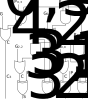
\includegraphics[width=0.95\textwidth]{lookahead_tree_carry.pdf}
\end{center}
\end{column}
\begin{column}{0.5\textwidth}

Doba výpočtu dvojic $G_{i,k}$ a $P_{i,k}$:
\begin{itemize}
\item Rychlost 4-ti bitových sčítanců 5 zpoždění hradel
\item Rychlost 8-ti bitových sčítanců 7 zpoždění hradel
\item Rychlost 64-ti bitových sčítanců 13 zpoždění hradel
\end{itemize}

\end{column}
\end{columns}

\end{frame}


\begin{frame}
\frametitle{Multiplexor}

Podobný přístup (rozděl a panuj - vytvoř stromovou strukturu) lze využít třeba i při konstrukci multiplexu:
\begin{columns}
\begin{column}{0.5\textwidth}
\begin{center}
   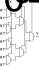
\includegraphics[width=0.5\textwidth]{multiplex-tree.pdf}
\end{center}
\end{column}
\begin{column}{0.5\textwidth}
\begin{itemize}
\item Podle tříbitového čísla $x$ se vybere odpovídající vstup $a_x$ na výstup $Y$
\item Není to nejrychlejší implementace, ale je přehledná
\item Můžeme využít i 4 vstupový multiplex a snížit počet úrovní stromu.
\end{itemize}

\end{column}
\end{columns}

\end{frame}

\begin{frame}[fragile,shrink=5]
\frametitle{Operace posun -- shift}

Oprace posun -- shift:
\begin{itemize}
\item Odpovídá to operaci jazyka C \texttt{>>} a \texttt{<<}
\begin{itemize}
\item Operace lze mimo jiné použít pro násobení mocninou 2 -- oprace \texttt{<<}; pro dělení mocninou 2 -- oprace \texttt{>>}
\end{itemize}
\item Jak implementovat posun o k-bitů?
\end{itemize}
\begin{columns}
\begin{column}{0.48\textwidth}
k-krát rotovat o 1 bit\\
Porovnej algoritmus mocnění:
\end{column}
\begin{column}{0.52\textwidth}
rotovat o 1, 2, 4, 8, 16 bitů\\
Porovnej algoritmus rychlého mocnění:
\end{column}
\end{columns}

\begin{columns}
\begin{column}{0.48\textwidth}
\begin{minted}{c}
double Exp(double a, int k) {
  if (k == 0) return 1;
  return a * Exp(a, k - 1);
}
\end{minted}
\end{column}
\begin{column}{0.52\textwidth}
\begin{minted}{c}
double FastExp(double a, int k) {
  if (k == 0) return 1;
  if (k % 2 == 0) {
    double i = FastExp(a, k / 2);
    return i * i;
  } else {
    return a * FastExp(a, k - 1);
  }
}
\end{minted}

\end{column}
\end{columns}



\end{frame}



\begin{frame}
\frametitle{Barrel shifter}

Rotaci o 0-7bitů lze složit z rotací o 1, 2, 4:
\begin{center}
   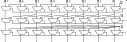
\includegraphics[width=0.75\textwidth]{barrel-shift.pdf}
\end{center}

\begin{itemize}
\item Multiplexory v každé řadě vybírají buď nedělej nic nebo posuň o daný počet bitů.
\item Bitové vstupy $x_2,x_1,x_0$ reprezentující binární číslo o kolik bitů rotovat
\item Příklad:
\begin{itemize}
\item posunutí o 5 bitů dostaneme složením posunutí o 1 bit a posunutí o 4 bity ($x_2=1$, $x_1=0$, $x_0=1$)
\item posunutí o 3 bity dostaneme složením posunutí o 1 bit a posunutí o 2 bity ($x_2=0$, $x_1=1$, $x_0=1$)
\end{itemize}
\end{itemize}

\end{frame}


\begin{frame}
\frametitle{Kvíz}

Kolik úrovní (řádek) Barrel shifter musí mít pro 64 bitové číslo, tedy pro rotace od 0 do 63?
\begin{itemize}
\item[A] 4
\item[B] 6
\item[C] 16
\item[D] 64
\end{itemize}

\end{frame}


\begin{frame}
\frametitle{Testovací kvíz}

Kolik jste toho dnes pochopili?
\begin{itemize}
\item[A] Vše bez problému.
\item[B] Téměř vše.
\item[C] Téměř nic.
\item[D] Vůbec nic.
\end{itemize}

\end{frame}


\end{document}

